\documentclass[12pt, block=fill]{beamer}
\usepackage[sfdefault]{FiraSans}
\usepackage{FiraMono}
\usepackage[T1]{fontenc}
\usepackage{xcolor}

\usepackage{pgfpages}
\setbeameroption{hide notes} % Only slides
% \setbeameroption{show only notes} % Only notes
 % \setbeameroption{show notes on second screen=right} % Both

\definecolor{burntOrange}{rgb}{.8, .5, .1}
\definecolor{textgray}{rgb}{.8,.8,.8}

\usetheme[titleformat frame = smallcaps]{metropolis}

\metroset{block=fill}

\newcommand{\E}{\text{E}}
\newcommand{\V}{\text{V}}
\newcommand{\cov}{\text{cov}}

\begin{document}

\section{Practical Significance of the T-Test}
\begin{frame}
  \frametitle{Practical Significance for the T-Test}

  After using a t-test to assess statistical significance, it is
  important to assess practical significance. \\ \vspace{1em}

  \begin{quote}
    Your main goal is to explain to your audience
    why they should or should not care about the effect.
  \end{quote}

  \textbf{Three common effect size measures:}

  \begin{enumerate}
  \item Difference in means
  \item Cohen's d
  \item Correlation r
  \end{enumerate}
\end{frame}

\begin{frame}
  \frametitle{Difference in Means}

  \begin{block}{Difference in means}
    \[
      \bar{X}_{A} - \bar{X}_{B}
    \]
  \end{block}
    \begin{itemize}
    \item Answers the question ``\textit{How different are these
        groups?''}
    \item Often makes great headlines
      and is a good choice if units are familiar
    \item But lacks context in its calculation
  \item People who eat chocolate live 1.5 years longer than those who
    do not each chocolate
  \end{itemize}
\end{frame}


  \begin{frame}
    \frametitle{Cohen's d}

    \begin{block}{Cohen's d}
      \small
    \textit{Cohen's d} is a measure of difference of means
    standardized by the variance in the data.
    \[
      \frac{ \bar{X}_{A} - \bar{X}_{B} }{s}
    \]
    Where $s$ is a pooled standard deviation:
    $\sqrt \frac{(n_1-1)s_1^2 + (n_2-1)s_2^2}{n_1+n_2}$
  \end{block}

  \begin{itemize}
  \item Answers the question ``\textit{How many standard
      deviations apart are the groups?}''
  \item The difference in sarcasm score between frequentists and
    Bayesians is $d = 0.54$ standard deviations.
  \end{itemize}
\end{frame}

\begin{frame}
  \frametitle{Correlation}
  \note[item]{Notice the similarity in the form between Cohen's d and
    correlation -- Cohen's d divides by the pooled standard deviation;
    correlation divides by the product of two group standard
    deviations.}
  \begin{block}{Correlation}
    \textit{Correlation} answers the question ``How strong is the
    relationship between group identity and the outcome?''
    \[
      \rho = \frac{\cov(X, Y)}{\sigma_{X}\sigma_{Y}}
    \]
  \end{block}

  \begin{center}
    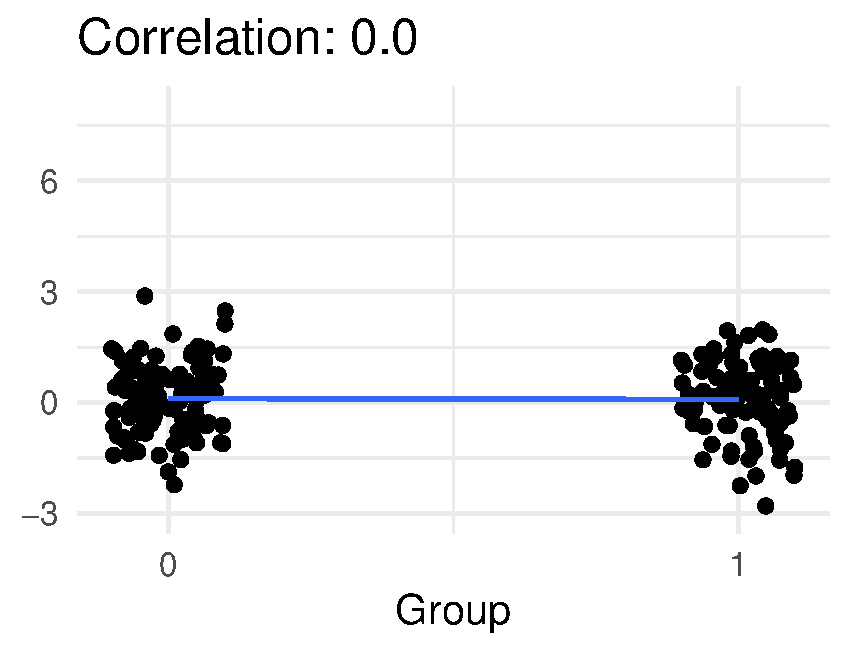
\includegraphics[width = 0.5\linewidth]{./figures/biserial_00}
  \end{center}
\end{frame}

\begin{frame}
  \frametitle{Correlation}

  \begin{block}{Biserial correlation}
    \textit{Correlation} answers the question ``How strong
    is the relationship between group identity and the outcome?''
    \[
      \rho = \frac{\cov(X, Y)}{\sigma_{X}\sigma_{Y}}
    \]
  \end{block}

  \begin{center}
    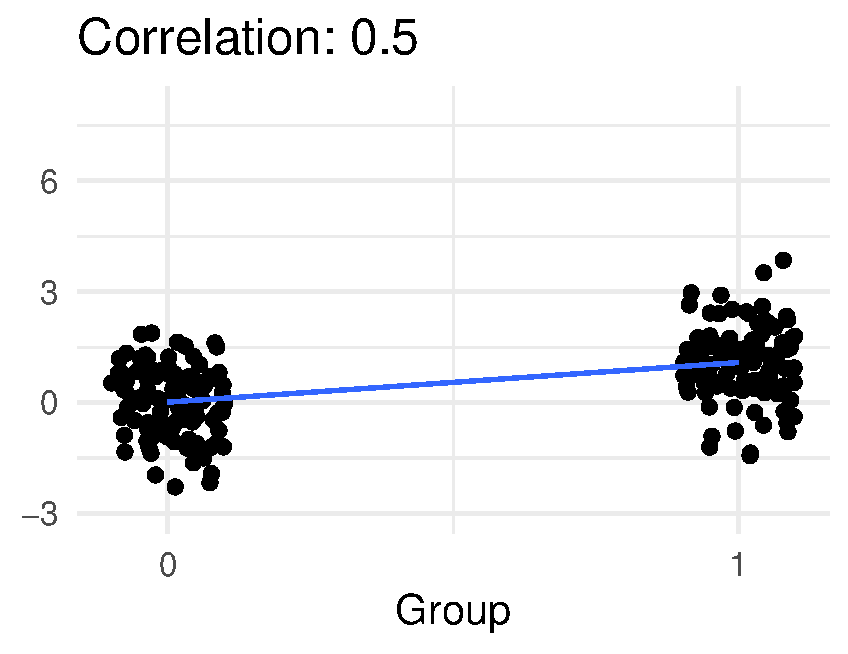
\includegraphics[width = 0.4\linewidth]{./figures/biserial_05}
  \end{center}
\end{frame}

\begin{frame}
  \frametitle{Correlation}

  \begin{block}{Biserial correlation}
    \textit{Correlation} answers the question ``How strong
    is the relationship between group identity and the outcome?''
    \[
      \rho = \frac{\cov(X, Y)}{\sigma_{X}\sigma_{Y}}
    \]
  \end{block}

  \begin{center}
    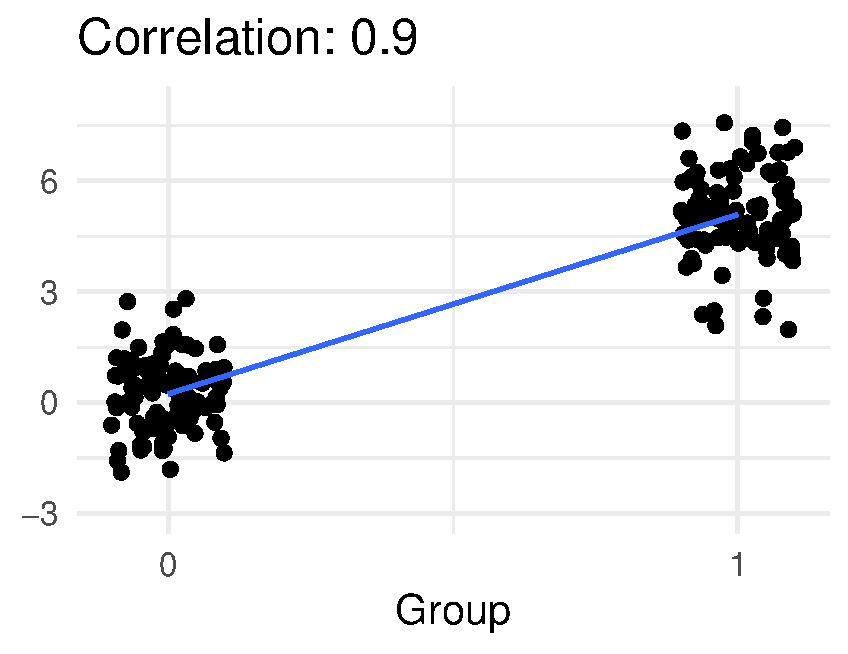
\includegraphics[width = 0.4\linewidth]{./figures/biserial_09}
  \end{center}
\end{frame}

\begin{frame}
  \frametitle{Practical Significance is about Context}

  \begin{itemize}
  \item How strong is the same relationship between \textit{different}
    groups?
  \item How strong is a \textit{different} relationship between the
    same group?
  \item What is the underlying dispersion in the data?
  \item What is a meaningful anchor or reference point that you can
    use for context?
  \end{itemize}
\end{frame}

\section{The Paired t-Test}

\begin{frame}
  \frametitle{Paired t-Test}

  \begin{exampleblock}{Climbing grip}
    Suppose you randomly sample 30 Berkeley students.  For each
    student $i$, you measure right-hand strength ($R_i$) and left-hand
    strength ($L_i$).

    \begin{itemize}
    \item You conduct a t-test with $H_0: \E[R] = \E[L]$
    \item \textbf{Problem}: Grip strength varies a lot
      person-to-person, $\Rightarrow$  t-test has low power.
    \end{itemize}
  \end{exampleblock}
\end{frame}

\begin{frame}
  \frametitle{Paired t-test}
  \centering
  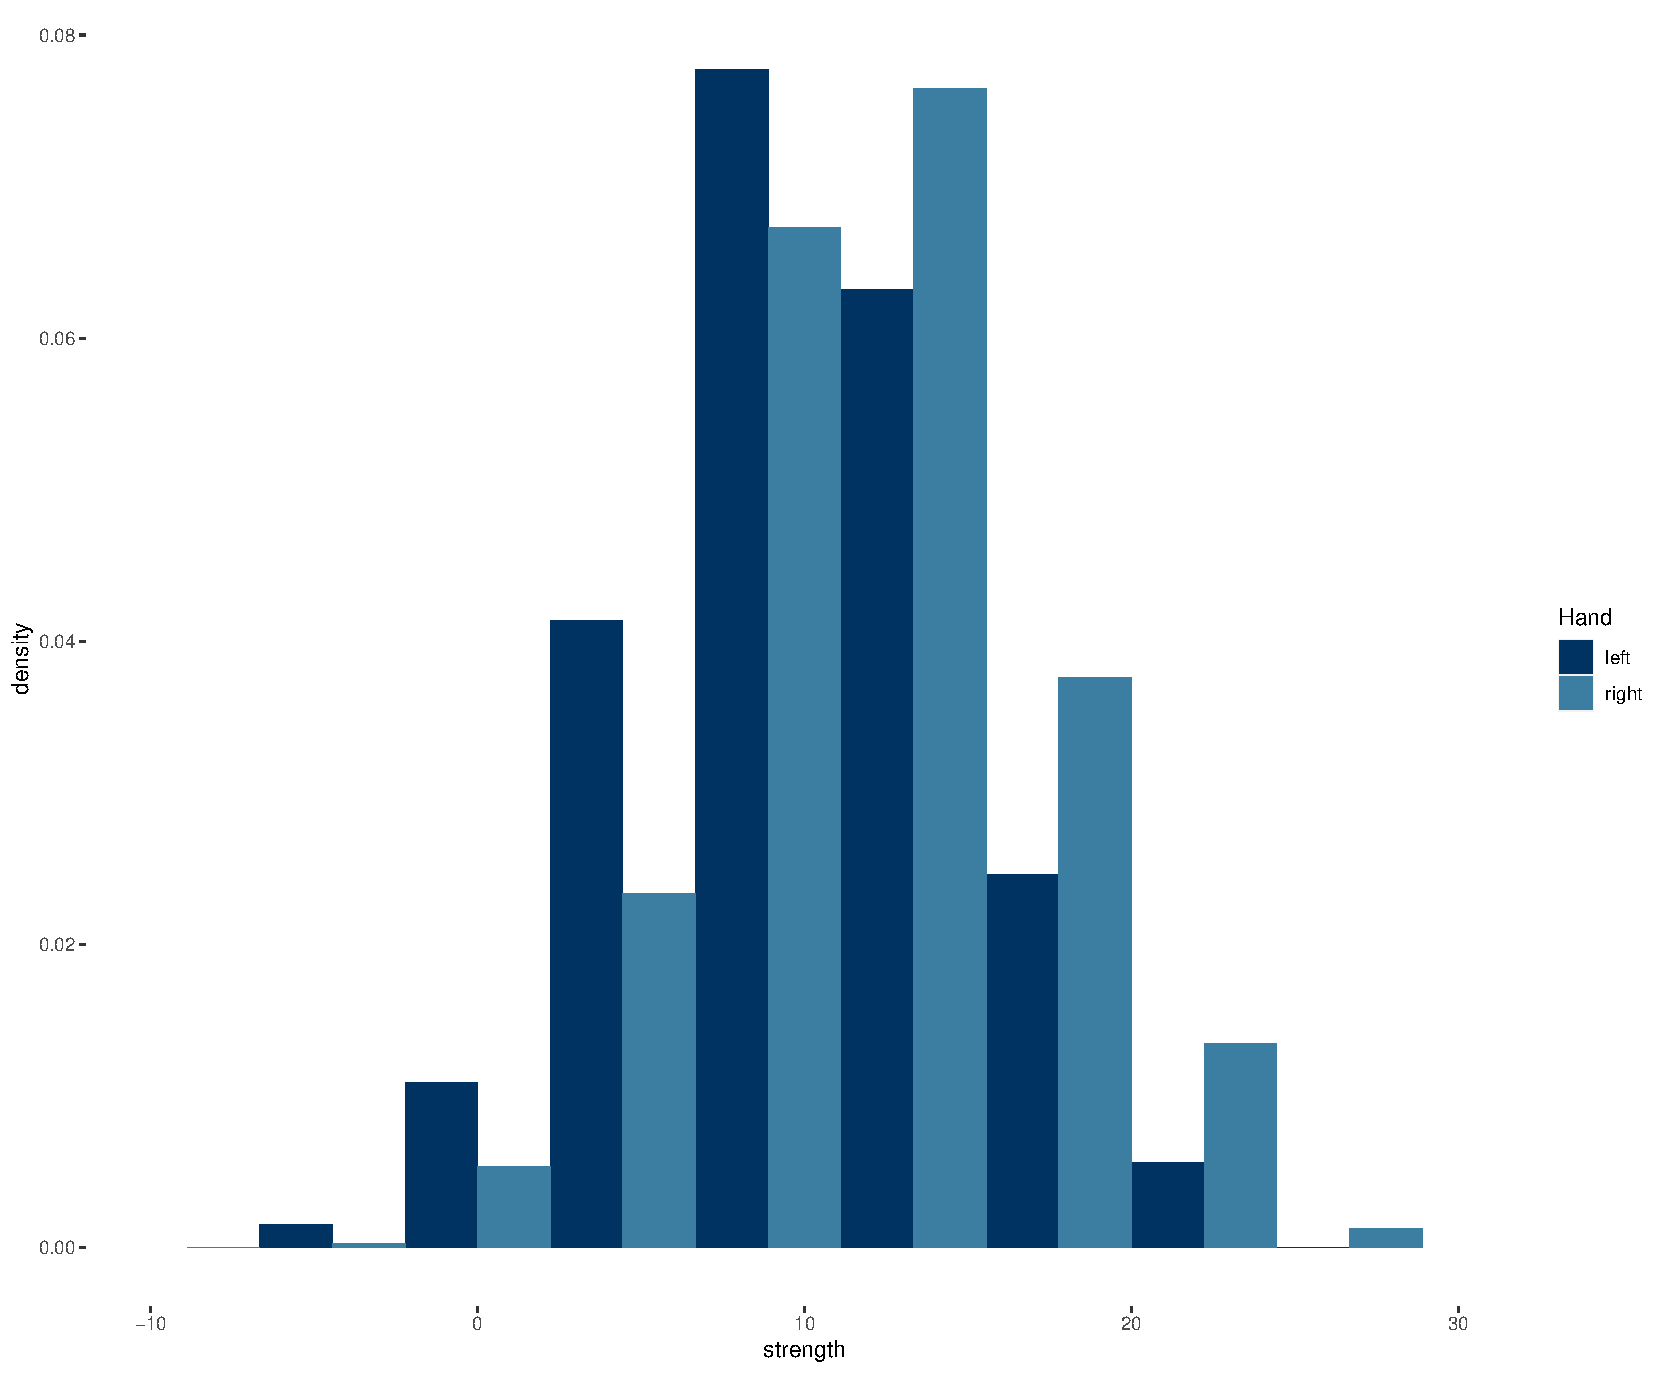
\includegraphics[width=.9\linewidth]{./figures/histogram_unpaired.pdf}
\end{frame}

\begin{frame}
  \frametitle{Paired t-Test}

  \begin{itemize}
  \item \textbf{Idea:} For any \textit{particular} subject $i$, the difference
    between right-hand strength and left-hand stregth, $R_i - L_i$,
    will usually be small.
  \item Within-person variation is small.
  \end{itemize}

  \begin{center}
    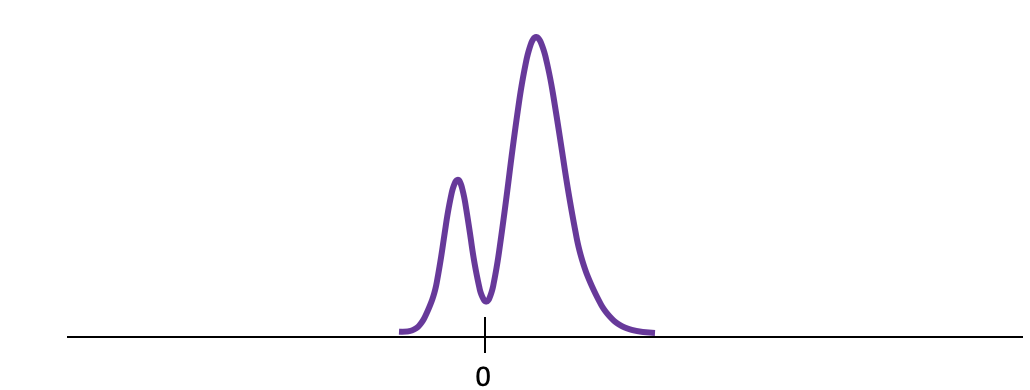
\includegraphics[width=.9\linewidth]{./figures/grip}
  \end{center}
\end{frame}

\begin{frame}
  \frametitle{Paired t-Test}
  \centering
    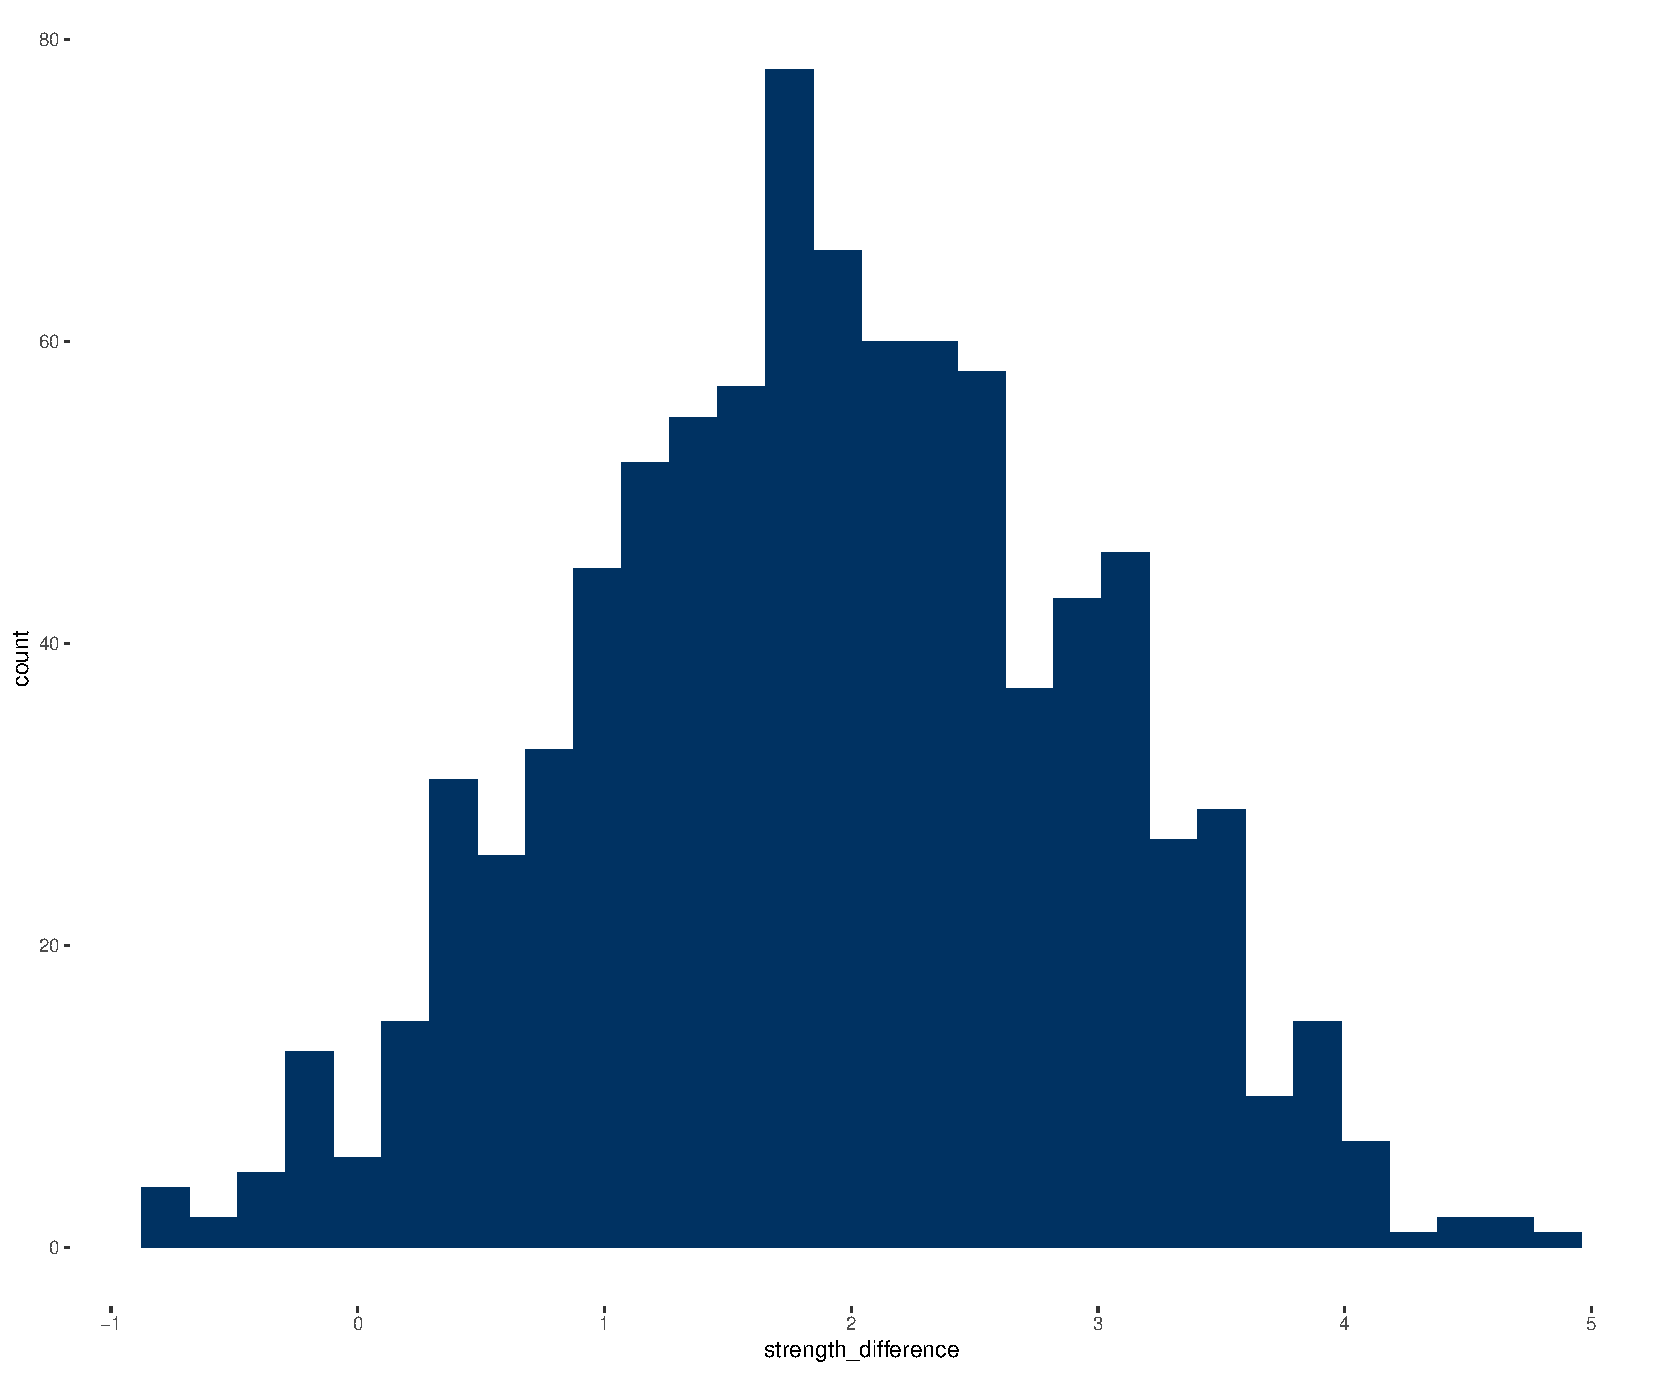
\includegraphics[width=.9\linewidth]{./figures/histogram_paired.pdf}
\end{frame}

\begin{frame}
  \frametitle{Paired t-Test}
  \centering
    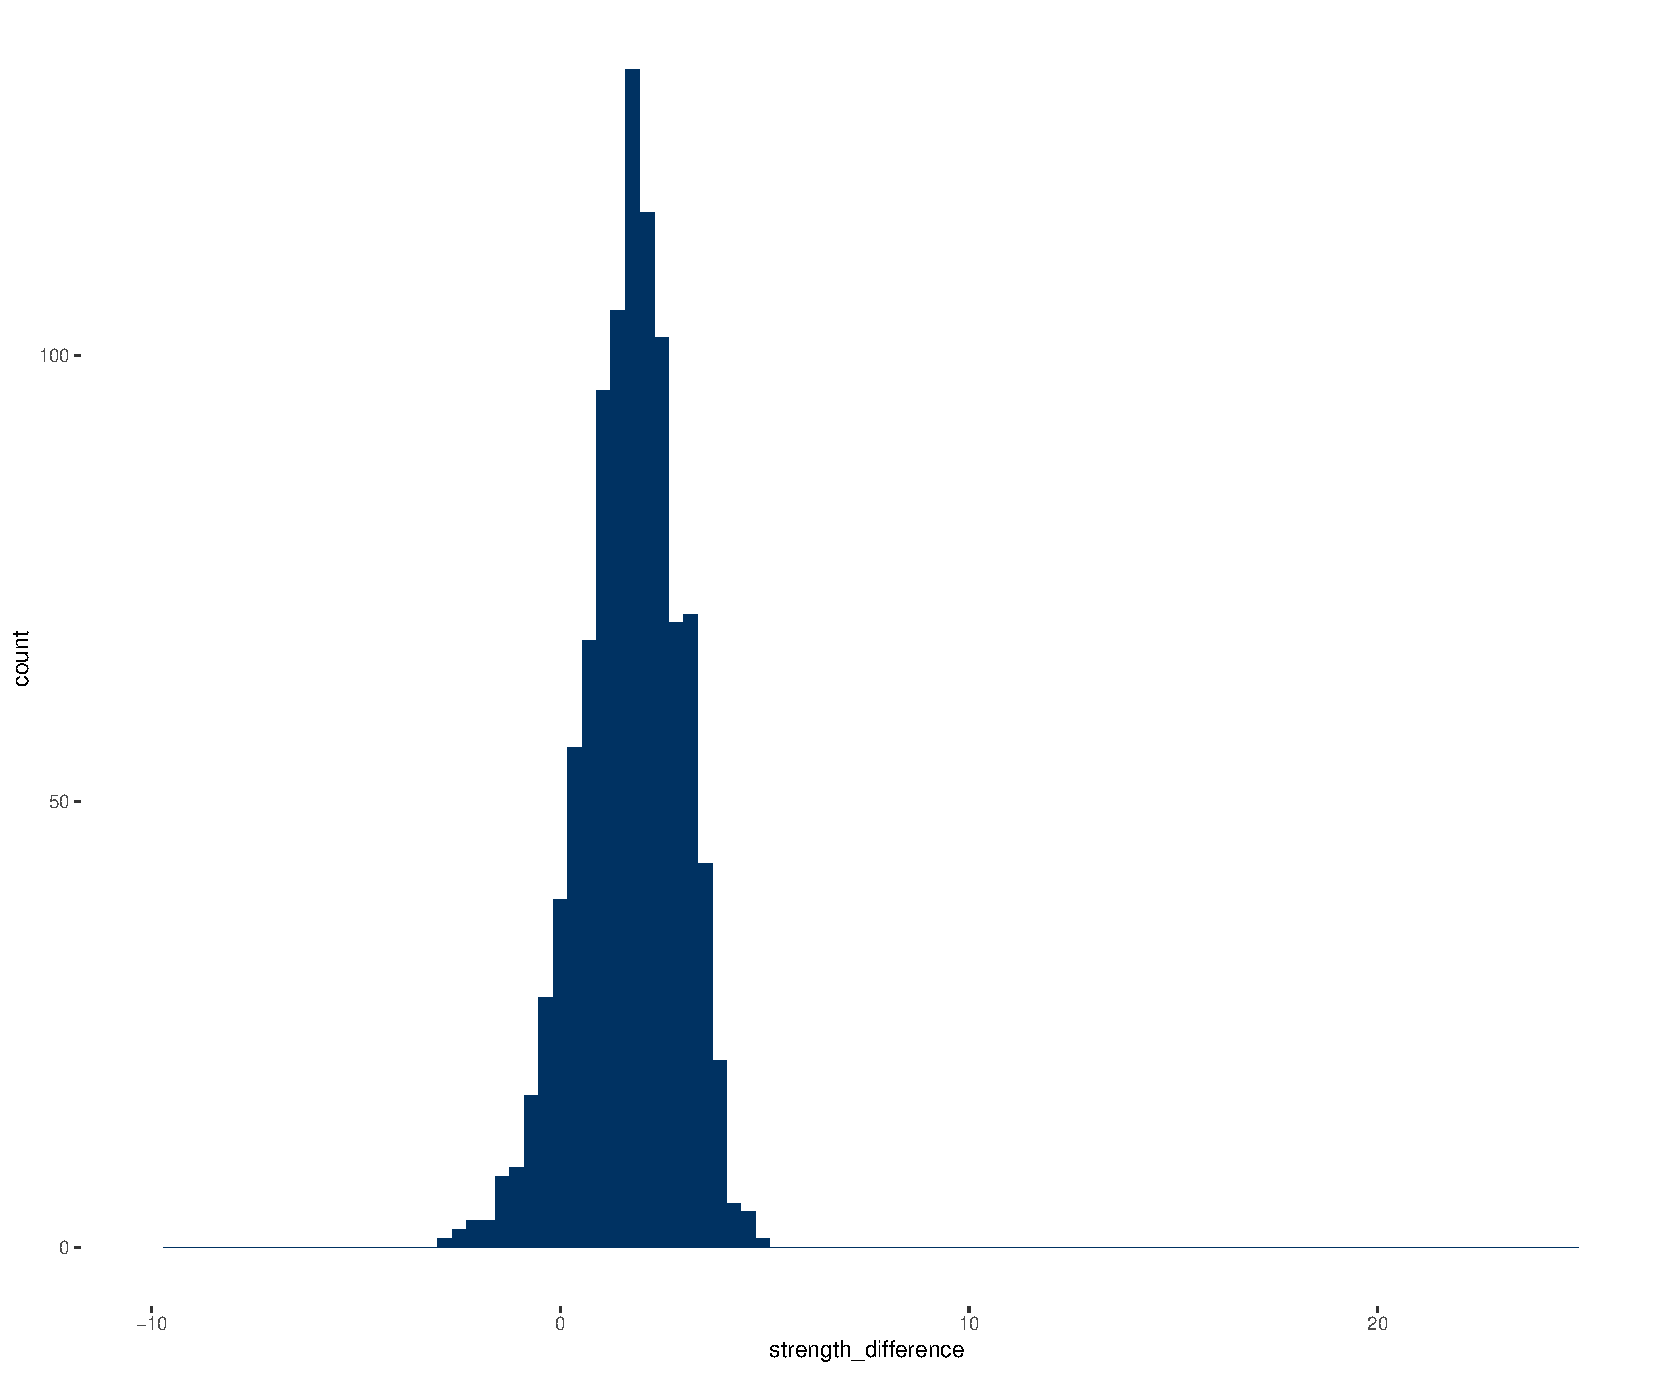
\includegraphics[width=.9\linewidth]{./figures/histogram_paired_rescaled.pdf}
\end{frame}

\begin{frame}
  \frametitle{Paired t-Test}
  \begin{block}{Paired t-test}
    A \textit{paired t-test}, sometimes called a \textit{dependent
      t-test}, builds an explicit dependency between data.
    Instead, perform a one-sample t-test with $H_0: \E[ R_{i}- L_{i}] = 0$.
  \end{block}
  \begin{itemize}
  \item This dependency must actually exist
  \item Cannot simply change the test
  \end{itemize}
\end{frame}

\begin{frame}
  \frametitle{Unpaired vs. Paired t-Test}

  \begin{columns}[t]
    \column{.49\linewidth}
    \textbf{Unpaired}
    \begin{itemize}
      \item $t = \frac{\bar{A} - \bar{B}} {\sigma_{A\&B}}$
    \end{itemize}
    \column{.49\linewidth}
    \textbf{Paired}
    \begin{itemize}
    \item $t = \frac{\bar{A} - \bar{B}}{\sigma_{(A - B)}}$
    \end{itemize}
  \end{columns}

\end{frame}

\begin{frame}
  \frametitle{Paired t-Test Assumptions}

  \begin{itemize}
  \item $A$ and $B$ have a metric scale with the same units.
  \item There is a natural pairing between observations for $A$ and for $B$.
    \begin{itemize}
    \item pre-test and post-test for same individual
    \item response to two types of stimulus for same mouse
    \item responses for a pair of spouses
    \end{itemize}
  \item Each pair $(A_i, B_i)$ is drawn i.i.d.
  \item The distribution of $A-B$ is sufficiently normal given the sample size.

  \end{itemize}
\end{frame}


\end{document}
